
\section{Durchführung}
\label{sec:durchfuerung}

Um die Fahrweisen in Reihen- und Parallelschaltung miteinander vergleichen zu können, würden im Präsenspraktikum verschiedene Druck-, Temperatur und Volumenstrommessungen für den warmen und den kalten Strom durchgeführt werden. Die Volumenströme werden dabei mittels Schwebekörperdurchflussmesser gemessen und über Ventile eingestellt.  Für die Druck- und Temperaturmessungen ist für das System jeweils der stationäre zustand abzuwarten.
Der schematische Versuchsaufbau, sowie das Schema der Ventile sind in den Abbildungen \ref{fig:schema} und \ref{fig:schema1} dargestellt.
\vspace{2mm}

\begin{figure}[h!]
	\centering
	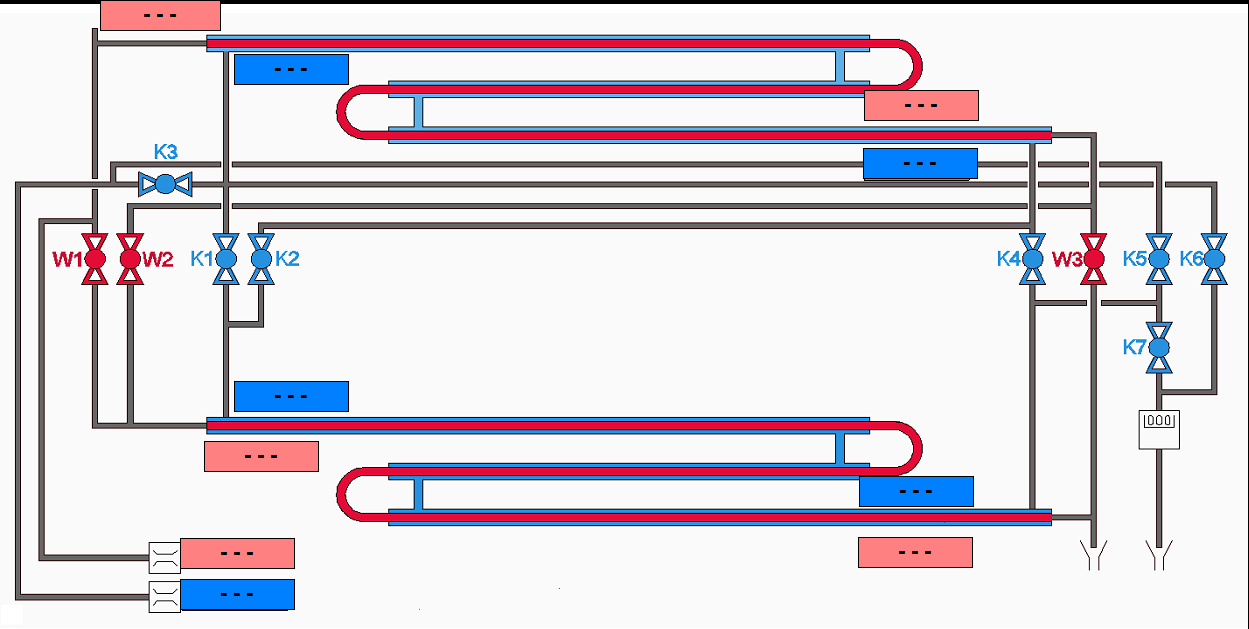
\includegraphics[width=0.7\textwidth]{img/schema}
	\caption{Schematische Darstellung der Ventile}
	\label{fig:schema}
\end{figure}
\FloatBarrier
%Ende
\begin{figure}[h!]
	\centering
	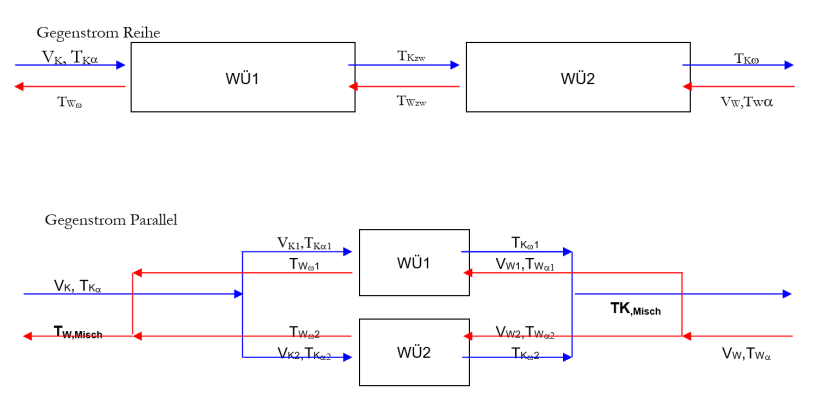
\includegraphics[width=0.75\textwidth]{img/schema1}
	\caption{Schematische Darstellung des Versuchsaufbaus}
	\label{fig:schema1}
\end{figure}
\FloatBarrier
%Ende